\newpage

\section{Crystal structure of Zircon/Zirconium(IV)silicate (ZrSiO4)}
\label{sec:ZrSiO4}

The peak profiling for the data for Zircon was done using the le Bail-wizard from \textit{Jana2006}. Here, the profiling was not ideal: Due to the $K\alpha$ doublet each peak consisted of two subpeaks. Strangely, the distance between the $2\theta$ values of those two peaks did not match the calculated $2\theta$-distance between the $K\alpha$ lines. Therefore, the fitting algorithm calculated basically one pseudo-Voigt curve for each peak instead of a composition of two [Fig. \ref{fig:demoShitPeaks}] and the wRp value never fell below 30. Anyhow, we continued refining the structure using the Rietveld-wizard of \textit{Jana2006}. The refined parameters are
\begin{gather*}
    \boxed{a = b = 6.608\,\mathrm{\AA} \quad c = 5.988\,\mathrm{\AA}}~.
\end{gather*}
The result is the profile shown in Fig. \ref{fig:ZrSiO4Prof}. In this Figure it can be clearly seen, that the profiling was not completely successful since the plot of the difference shows a few very high values near the peaks. This could either be due to an unskilled usage of \textit{Jana2006} or an unknown variation in the setup. In spite of this, the structure of Zircon [Fig. \ref{fig:ZrSiO4Struct}] aligns to the Ref. \citenum{Hanchar2003}. The typical ZrO\textsubscript{8} trigondodecahedra and the SiO\textsubscript{4} tetrahedra are highlighted in the polyhedral figure style. 

\begin{center}
    \begin{sidewaysfigure}
    \centering
    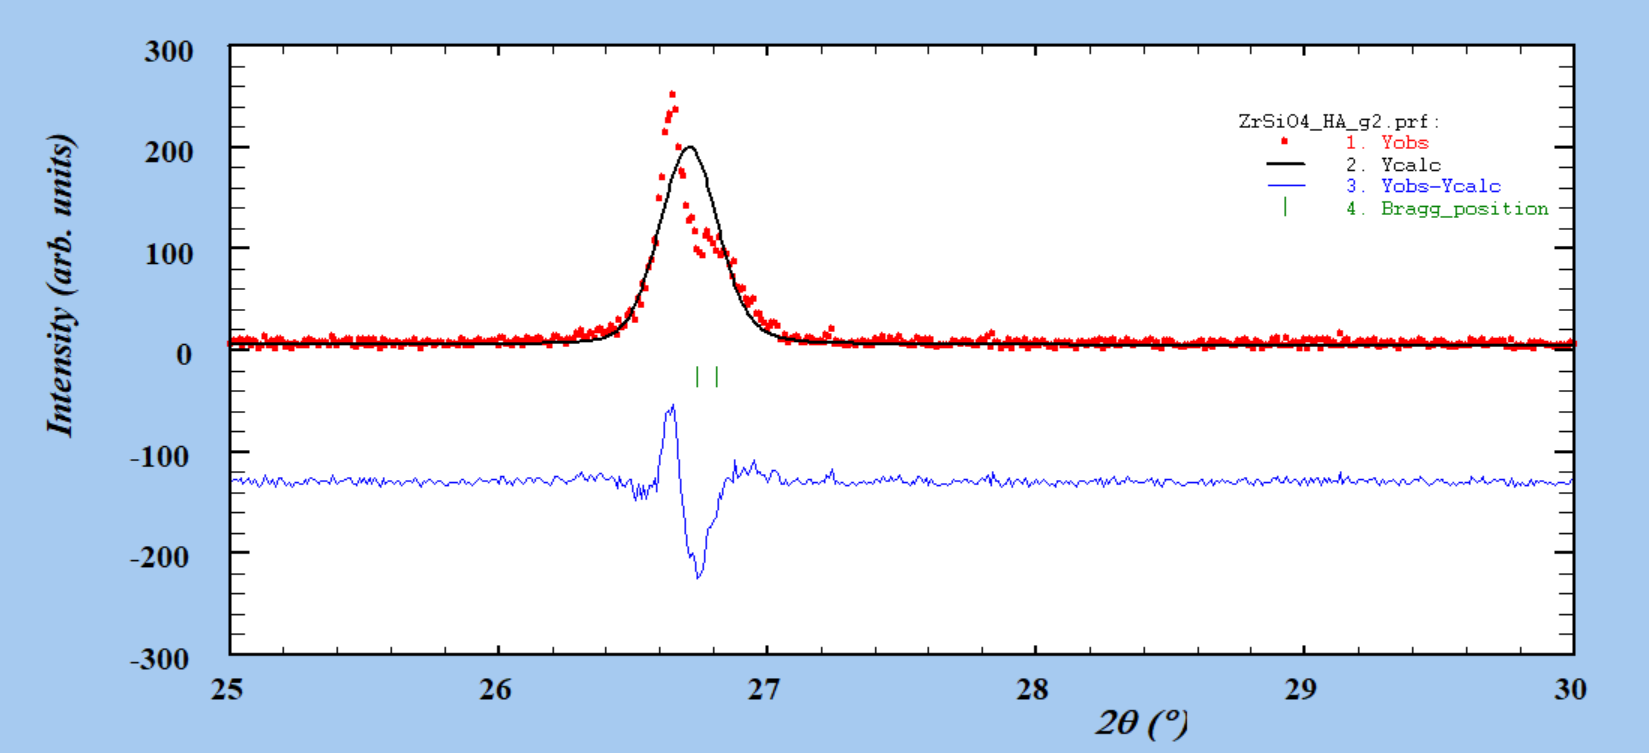
\includegraphics[width = 0.9\textheight]{Pictures/Evaluation/43/ZrSiO4DemoPeak.png}
    \caption{
        Due to the different distances between the $K\alpha$ lines and the two subpeaks of each peak, the profile could not be calculated exactly, but just as one pseudo-Voigt curve instead of a composition of two.
    }
    \label{fig:demoShitPeaks} 
    \end{sidewaysfigure}
\end{center}

\begin{center}
    \begin{sidewaysfigure}
    \centering
    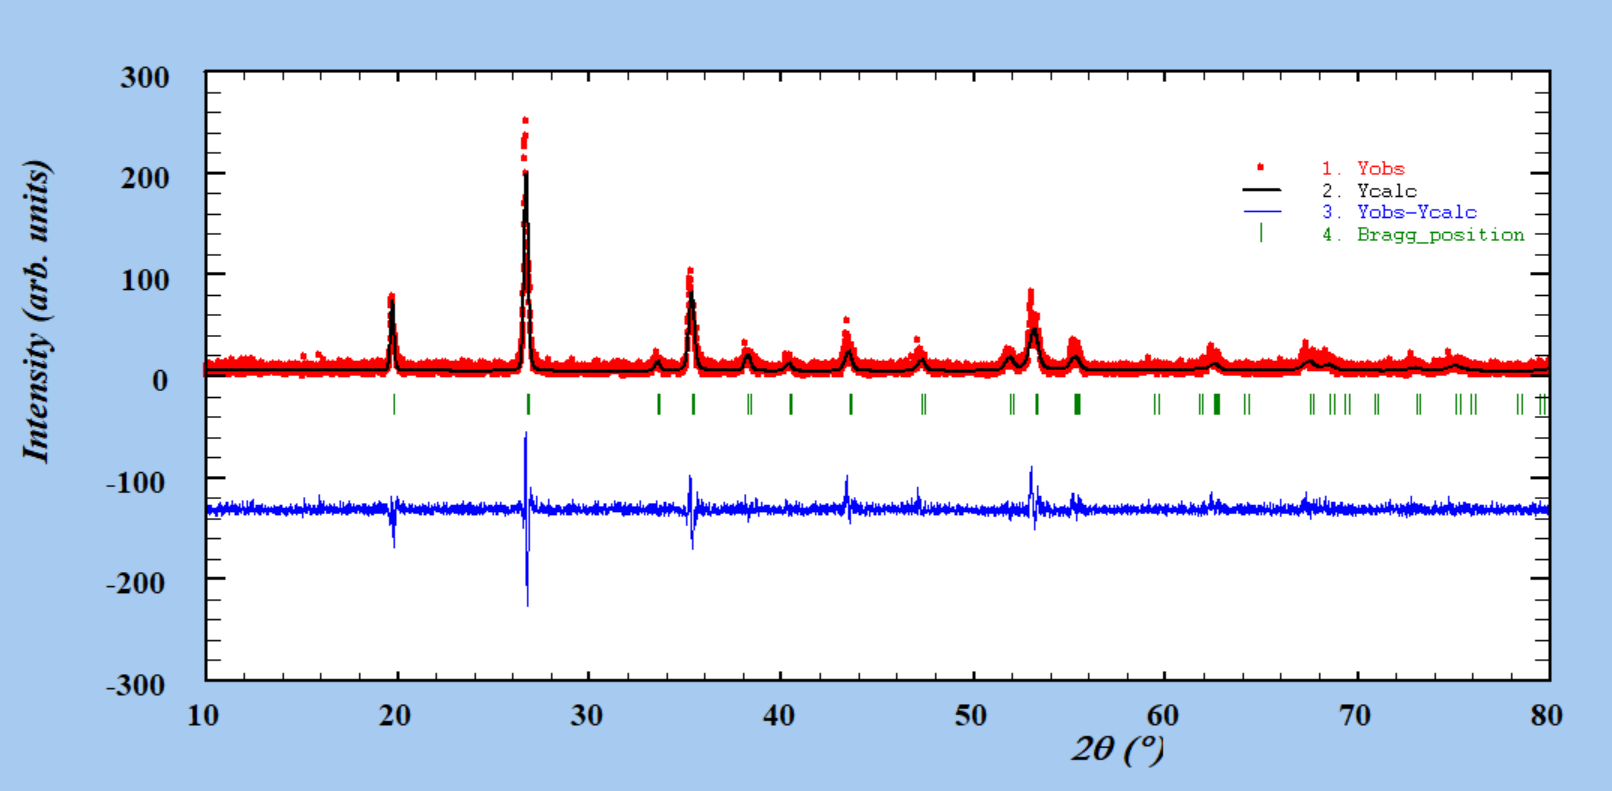
\includegraphics[width = 0.9\textheight]{Pictures/Evaluation/43/ZrSiO4DataAll.png}
    \caption{
        For the Zircon data in red, the whole calculated profile is shown in black and the difference curve in blue.
    }
    \label{fig:ZrSiO4Prof}
    \end{sidewaysfigure}
\end{center}

\begin{center}
    \captionsetup{type = figure}
    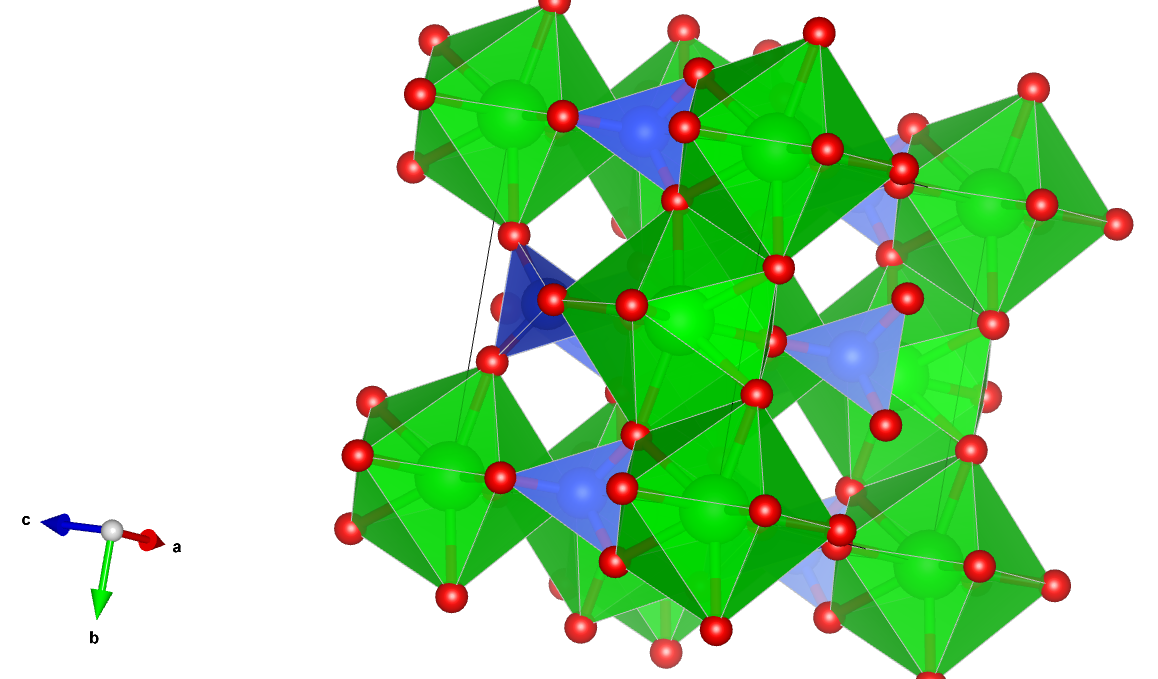
\includegraphics[width = 0.7\textwidth]{Pictures/Evaluation/43/ZrSiO4StructurePolyhedral.png}
    \captionof{figure}{
        A model of the refinded Zircon structure is shown in a polyhedral style. Here, the typical ZrO\textsubscript{8} trigondodecahedra (in green) and the SiO\textsubscript{4} tetrahedra (in blue) can be seen. 
    }
    \label{fig:ZrSiO4Struct}
\end{center}
